\documentclass[11pt]{article}

\usepackage{amssymb,amsmath,amsthm} 
\usepackage{datetime}
\usepackage[margin=1.25in]{geometry}
\usepackage{graphicx,ctable,booktabs}
\usepackage{fancyvrb}
\usepackage{units}
\usepackage{enumerate}
\usepackage{tikz}

\usepackage{fancyhdr}
\pagestyle{fancy}
\fancyhf{}
\lfoot{\small\scshape Qiming Fang (qf26)} 
\cfoot{\small\scshape \thepage} 
\rfoot{\small\scshape \footnotesize  INFO 4300 - Assignment 1} 
\renewcommand{\headrulewidth}{0pt}
\renewcommand{\footrulewidth}{.3pt}

\newcounter{ctFigures}
\setcounter{ctFigures}{1}

\begin{document}

\title{\textbf {INFO 4300 - Assignment 1}}
\author{Qiming Fang (qf26)}
\date{\today}

\maketitle
\thispagestyle{fancy}
\section*{Logistics}
For this project, I decided to use python 2.7.2. Included should be a \emph{data} directory, a \emph{stoplist.txt} file, a \emph{main.py} file, and this documentation.
\section*{Index Design}
Since python doesn't natively support trees, I decided to implement my own binary serach tree using custom data structures. For example, I defined a custom class, \textbf{TreeNode}, which represents a node in this binary tree. It has a pointer to each of its left and right children, as well as a third pointer to an instance of the \textbf{Postings} class. Note that the left and right children could be None.
\begin{center}
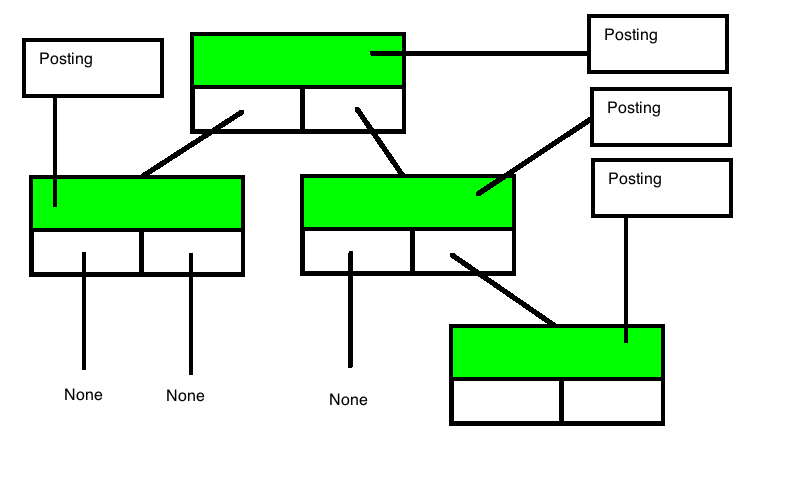
\includegraphics[scale=0.5]{treeNode}
\begin{flushright}
\underline{Figure \arabic{ctFigures}:} Visual representation of a TreeNode inside the index.
\addtocounter{ctFigures}{1}
\end{flushright}
\end{center}
An instance of \textbf{Tree}, therefore, is simply a structure that contains a pointer to the root TreeNode. In addition, a Tree supports many operations on the nodes in the tree, such as:
\begin{Verbatim}[frame=single]
# inserts given string into the tree, along with which file it was found,
# the position inside the file, and a short description
def insert(self, string, filename, loc, desc)
\end{Verbatim}
\begin{Verbatim}[frame=single]
# finds the given string inside the tree. Returns a treeNode or None
def find(self, str)
\end{Verbatim}
An Instance of the \textbf{Postings} class contains information about a particular indexed term, such as which files contain it, where in the files is it found, along with a short snippet of the context in which this term appears.
\begin{center}
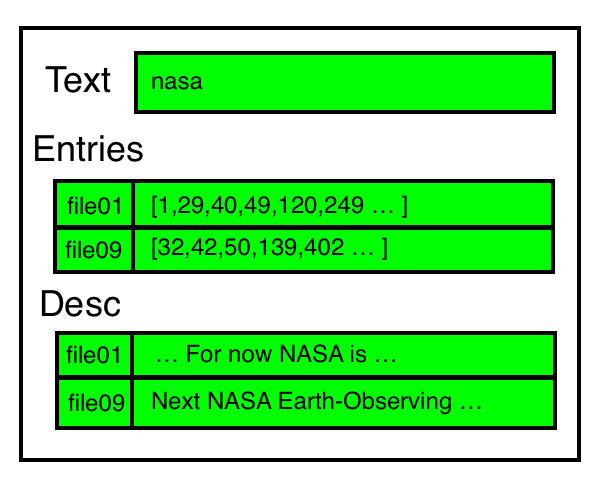
\includegraphics[scale=0.6]{posting}
\begin{flushright}
\underline{Figure \arabic{ctFigures}:} A Postings file - used to keep track of indexing information
\addtocounter{ctFigures}{1}
\end{flushright}
\end{center}
Structuring the Postings file like this makes it very easy to calculate \emph{tf} and \emph{idf} values. \emph{idf} can be calculated by 1 + log (N/(len(entries))). \emph{tf} can be calculated by first looking up $f_{i,j}$ - i.e. len(entries[filename]) - and calculating 1 + log($f_{i,j}$).
\section*{Query Processing}
When a user inputs a query, the program first checks whether the user entered a single word query or a multi-word query. If a single word query was issued, then it probes the index to find the right postings file, calculate tf/idf scores, then prints the relevant information. If a multi-word query was issued, it probes the index multiple times to generate, for each term, a list of documents that contains the term. It then runs a map function and a merge function to find the intersection between these lists. \\

\noindent
Once it has the list of documents that contain every term, the program runs through again and calculates the sum of the tfidf scores in a document (for all of the terms), and then sorts them by tfidf scores in reverse. For details, please consult specific comments in source code.
\section*{Design Decisions}
\begin{enumerate}
\item Trees can quickly become unbalanced. I included an AVL implemenation with the code. Users can include the -a flag to run with an AVL tree. This means that inserts will take longer -- O(nlogn) instead of O(logn), but it ensures an O(logn) lookup time.
\item I've chosen to cache 10 neighboring words in memory, rather than fetching the 10 neighboring terms everytime. This approach saves the round trip time of retrieving files from disk every time; however, more memory is consumed for the index.
\item By using a tree, my program can support range queries, since all entries are sorted by the BST invariant
\item The index can support (althought not implemented) addition and deletion operations. 
\end{enumerate}
\section*{How to Run Code}
To run with normal BST index:
\begin{Verbatim}[frame=single]
python main.py -d data -s stoplist.txt
\end{Verbatim}
To run with AVL tree index:
\begin{Verbatim}[frame=single]
python main.py -d data -s stoplist.txt -a
\end{Verbatim}
\end{document}